\section{Silniki magazynu danych}
Architektura MySQL umożliwia korzystanie z wielu różnych silników, które są  odpowiedzialne za wykonywanie operacji na danych. Silnik bazy danych wybierany jest per tabela, co oznacza, że w ramach pojedynczej bazy danych można używać różne silniki.
\subsection{Krótka charakterystyka podstawowych silników.}
W tym podrozdziale nie będę się skupiał na szczegółowym opisie większości z silników dostępnych w MySQL, postaram się raczej w ogólny sposób przedstawić ich główne charakterystyki, zalety oraz ograniczenia. Część z silników została pominięta ze względu na ich marginalną popularność oraz zastosowanie. Na wstępie chciałbym podkreślić fakt, że w zdecydowanej większości przypadków najodpowiedniejszym aktualnie silnikiem jest InnoDB, aczkolwiek każdy z silników opisanych w tym rozdziale ma pewne zalety i w specyficznych przypadkach, które przedstawiłem w tym rozdziale, warto rozważyć użycie silnika alternatywnego do InnoDB.
\subsubsection{MyISAM}
MyISAM był domyślnym silnikiem składowania danych do wersji 5.4 (włącznie). Każda tabela przechowywana jest w dwóch plikach na dysku twardym. Dane przechowywane są w pliku z rozszerzeniem \textbf{.MYD (MYData)}
natomiast w drugim pliku (\textbf{.MYI(MYIndex)}) składowane są indeksy. Poniżej przedstawię kilka cech tego silnika bazy danych. 
\begin{itemize}
	\item \textbf{Brak wsparcia dla transakcji.} Z tego powodu MyISAM nie powinien być używany do tabel, dla których istotnym wymaganiem jest zapewnienie integralności danych.
	\item \textbf{Obsługa indeksów B-tree oraz Geospatial.}
	\item \textbf{Blokady tabeli.}  W momencie, kiedy wykonujemy operacje dodającą dane do tabeli, jest ona blokowana na cały czas wykonywania operacji (również dla operacji odczytujących dane). Sprawia to, że w przypadku dużej liczby operacji modyfikujących dane - wydajność bazy danych wyraźnie spada.
	\item \textbf{Brak obłusgi mechanizmu kluczy obcych}
	\item \textbf{Mechanizm kompresji danych.} Silnik umożliwia kompresowanie danych w celu optymalizacji ilości miejsca potrzebnego do przechowywania danych z tabeli. Taka operacja sprawia, że skompresowane dane są dostępne jedynie do odczytu, a ich modyfikacja jest zablokowana i wymaga rozpakowania danych. Tabele MyISAM można kompresować i dekompresować za pomocą mechanizmu \textit{myisampack}.
	\item \textbf{Buforowanie indeksów.} Silnik MyISAM buforuje jedynie indeksy.
	\item \textbf{Obsługa statystyk.}
\end{itemize}

W czasie pisania tej pracy silnik MyISAM nie był już praktycznie rozwijany, dlatego raczej odradzam jego stosowanie w nowszych wersjach serwera MySQL. 

\subsubsection{InnoDB}
Od wersji 5.5 InnoDB jest domyślnym silnikiem bazy danych MySQL. Mechanizm InnoDB został uzupełniony o funkcje, których brakowało w MyISAM i obecnie jest zdecydowanie najpopularniejszym wyborem. Domyślnie dane przechowywane są w pojedynczych plikach, ale możliwe mogą być również przechowywane w wielu plikach. Struktura plików bazy \textit{StackOverflow}, która dla wszystkich tabel używa silnika InnoDB, została przedstawiona na rysunku ~\ref{fig:innodb-fileslabel}.
\begin{figure}
	\caption{Pliki silnika InnoDB testowej bazy danych \textit{StackOverflow}}
	\centering
	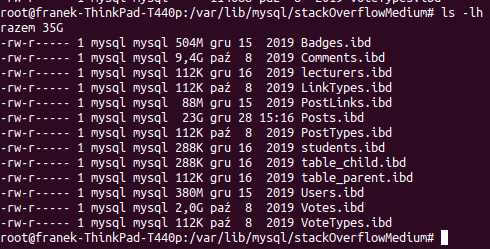
\includegraphics[scale = 0.43]{innodb-files.png}
	\label{fig:innodb-fileslabel}
\end{figure}
Poniżej przedstawiłem kilka podstawowych charakterystyk silnika.
\begin{itemize}
	\item \textbf{Wsparcie dla transakcji.} Silnik wspiera transakcje oraz cztery poziomy izolacji.
	\item \textbf{Wsparcie dla indeksów.} InnoDb wspiera najważniejsze indeksy takie jak: B-tree, Hash, Spatial.
	\item \textbf{Blokowanie dostępu na poziomie rekordów. } Dostęp do tabel InnoDB jest blokowany za pomocą mechanizmy MVCC (Multi-Versioned Concurrency Control), który w przeciwieństwie do MyISAM blokuje pojedyncze rekordy, zamiast całej tabeli. Wprowadzenie tej zmiany znacząco zwiększyło wydajność równoległych operacji modyfikujące dane w tabeli.
	\item \textbf{Wsparcie dla kluczy obcych.}
	\item \textbf{Buforowanie danych oraz indeksów.} Silnik InnoDb może buforować nie tylko indeksy, ale również dane.
	\item  \textbf{Nieskompresowane indeksy.} Silnik InnoDb nie kompresuje indeksów, co prowadzi do zwiększenia zużycia przestrzeni dyskowej.
	\item \textbf{Wsparcie dla partycjonowania.} Szerzej opisane w podrozdziale dotyczącym partycjonowania.
	\item \textbf{Obsługa statystyk.}
\end{itemize}

\subsubsection{CSV Storage Engine}
Silnik CSV Storage Engine przechowuje dane tabeli w plikach tekstowych w formacie csv z wartościami rozdzielonymi przecinkami.Ten silnik może być przydatny, jeżeli chcemy nasze dane przechowywać w formacie csv, ale posiada wiele ograniczeń, dlatego nie jest zalecane jego stosowanie, o ile nie zależy nam na przechowywaniu danych tabeli w formacie CSV.
Poniżej przedstawiłem kilka podstawowych charakterystyk silnika.
\begin{itemize}
	\item \textbf{Brak wsparcia dla indeksów i kluczy obcych.}
	\item \textbf{Brak wsparcia dla transakcji.}
	\item \textbf{Brak możliwości przechowywania wartości \textit{null}.}
	\item \textbf{Brak wsparcia dla partycjonowania.}
\end{itemize}

\subsubsection{Memory}
Tabele z silnikiem Memory są tabelami, których dane przechowywane są w pamięci, a nie na dysku twardym. Dane przechowywane w tabeli są ulotne i zostają usunięte w momencie restartu serwera (struktura tabeli zostaje zachowana). Z powodu przechowywania w pamięci są o rząd wielkości szybsze od standardowych silników baz danych, ale ze względu na swoją ulotność nie powinny przechowywać istotnych danych dla aplikacji.
Niżej przedstawiłem kilka podstawowych własności tabeli Memory.
\begin{itemize}
	\item \textbf{Wsparcie dla indeksów} Tabele Memory obsługują indeksy Hash oraz B-tree. Domyślnym indeksem jest indeks typ Hash.
	\item \textbf{Blokowanie na poziomie tabeli.} Podobnie jak tabele MyISAM, w momencie modyfikowania danych blokowana jest cała tabela.
	\item \textbf{Brak obsługi typów TEXT oraz BLOB}. Tabele nie obsługują typów TEXT. Przechowywanie teksu możliwe jest w kolumnach VARCHAR o stałej zdefiniowanej wielkości, co prowadzi do marnotrawienia pamięci.
	\item \textbf{Brak danych statystycznych indeksu.} Tabele MEMORY nie przechowują statystyk dotyczących indeksów, co czasami może skutkować wybraniem nieodpowiedniego indeksu przez optymalizator zapytań i w efekcie pogorszenie wydajności zapytań.
	\item \textbf{Brak wsparcia dla transakcji.}
\end{itemize}

 Poniżej wymieniłem kilka przypadków użyca tabeli z silnikiem Memory. 
\begin{itemize}
	\item Pamięć podręczna dla często odczytywanych danych, która jest wczytywana w momencie startu serwera.
	\item Buforowanie wyników agregowanych danych z często wykonywanych zapytań.
	\item Przechowywanie wyników pośrednich z zapytań.
	\item MySQL używa tabeli Memory do wewnętrznego przetwarzania zapytań wymagających tabeli tymczasowych do przechowywania wyników pośrednich.
\end{itemize}

\subsubsection{Silnik Archive}
Silnik archive służącym do przechowywania dużej ilości nieindeksowanych danych, które są rzadko pobierane. 

\begin{itemize}
	\item \textbf{Możliwe wykonywanie jedynie operacji INSERT, REPLACE oraz SELECT}. W tabelach Archive niemożliwe jest usuwanie i modyfikowanie istniejących krotek.
	\item \textbf{Brak wsparcia dla indeksów.}
	\item \textbf{Blokowanie na poziomie tabeli.}
	\item \textbf{Kompresowanie danych.} Każdy wstawiony rekord jest automatycznie kompresowany za pomocą \textit{zlib}, dlatego tabele Archive wymagają zdecydowanie mniej miejsca od tabel InnoDB lub MyISAM.
	\textit{Brak wsparcia dla transakcji.}
\end{itemize}


\subsection{Porównanie silników}



\subsubsection{Przechowywanie danych}
W celu porównania sposobu przechowywania danych na dysku, przygotowałem testową bazę danych, zawierającą pięć tabel będących niemalże kopią tabeli \textit{Users} z bazy testowej, z których każda wykorzystuje inny silnik. Jedyną zmianą jest brak kolumny \textit{AboutMe}, która została usunięta ze względu brak wsparcia dla kolumn TEXT w silniku MEMORY. Do tworzenia tabel wykorzystałem następujące polecenie, a następnie zaimportowałem dane z bazy \textit{Stackoverflow}. Ze względu na fakt, że nie wszystkie silniki wspierają przechowywania wartości NULL, zamieniłem domyślne wartości NULL na wartość 0 lub pustego tekstu (w zależności od typu danych).
\begin{spverbatim}
	CREATE TABLE `Users` (
	`Id` int NOT NULL,
	`Age` int NOT NULL DEFAULT 0,
	`CreationDate` datetime NOT NULL,
	`DisplayName` varchar(80) NOT NULL,
	`DownVotes` int NOT NULL,
	`EmailHash` varchar(80) NOT NULL DEFAULT '',
	`LastAccessDate` datetime NOT NULL,
	`Location` varchar(200) NOT NULL DEFAULT '',
	`Reputation` int NOT NULL,
	`UpVotes` int NOT NULL,
	`Views` int NOT NULL,
	`WebsiteUrl` varchar(400) NOT NULL DEFAULT '',
	`AccountId` int NOT NULL DEFAULT 0,
	PRIMARY KEY (`Id`) -- w tabelach, które wspierają klucze główne
	) ENGINE=<nazwa silnika>;
\end{spverbatim}
Dla silników, które nie wspierają kluczy głównych, musiałem je usunąć. Ostatecznie tabela zawiera w granicach 2,5 miliona wierszy. Silnik NDB pominąłem, ponieważ został dodatkowo opisany w rozdziale dotyczącym skalowalności.
\begin{figure}[!h]
	\caption{Baza danych użyta do testowania silników baz danych}
	\centering
	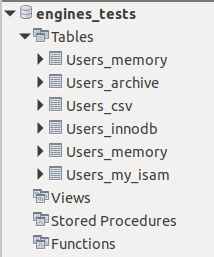
\includegraphics[scale = 0.59]{engines_tests.png}
	\label{fig:label}
\end{figure}
\begin{figure}[!h]
	\caption{Pliki z danymi użytkowników dla testowych silników.}
	\centering
	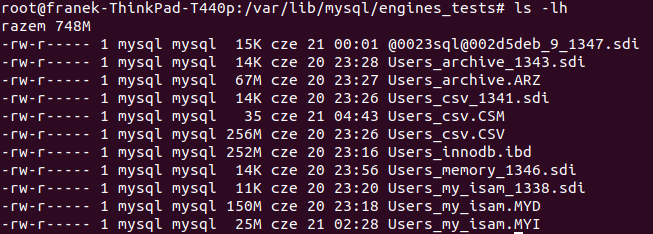
\includegraphics[scale = 0.6]{engines_storage.png}
	\label{fig:engines_storage}
\end{figure}
Jak możemy zauważyć na rysunku ~\ref{fig:engines_storage} pod względem optymalizacji ilości miejsca na dysku zdecydowanie najlepiej wypada silnik Archive, który potrzebuje jedynie 67 MB dla danych użytkowników. Na drugim miejscu pod tym względem plasuje się silnik MyISAM. Silniki InnoDB oraz CSV wymagają praktycznie takiej samej przestrzeni dyskowej; w granicach 250 MB. Silnik MEMORY na dysku twardym przechowuje jedynie strukturę tabeli, ale do sprawdzenia ilości użytej pamięci możemy użyć narzędzia \textit{MySQL Workbench}.
\begin{figure}[!h]
	\caption{Informacje dotyczące tabeli Users\textunderscore memory w \textit{MySQL Workbench}. \textit{StackOverflow}}
	\centering
	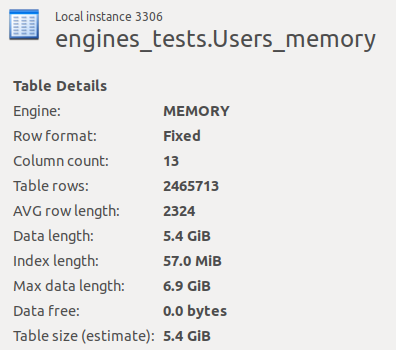
\includegraphics[scale = 0.6]{memory_engine_storage.png}
	\label{fig:label}
\end{figure}
Silnik MEMORY wymaga bez mała 5.5 Gb pamięci. Wynika to w dużej mierze z tego, że silnik MEMORY dla kolumn VARCHAR zawsze rezerwuje rozmiar wynikający z maksymalnej wartości, nawet jeżeli nie jest ona wykorzystana.




\subsubsection{Wymaganie transakcyjności}
W przypadku tabel, które wymagają użycia transakcji, jedynym możliwym wyborem jest silnik InnoDB.

\subsubsection{Operacje odczytu klucz-wartość}
Do testów użyłem narzędzia \textit{sysbench}, który posiada wbudowany mechanizm ułatwiający testowanie baz danych. Na początku przygotowałem testową bazę danych udostępnioną przez \textit{sysbench} za pomocą polecenia:
\begin{spverbatim}
	sysbench --db-driver=mysql --mysql-user=root --mysql-password=root --mysql-db=test --table_size=2000000 --range_selects=off --mysql_storage_engine=
	<nazwa silnika> /usr/share/sysbench/oltp_read_only.lua prepare
\end{spverbatim} 
Baza danych zawiera 2 miliony rekordów, tabela domyślnie przyjmuje nazwę \textit{sbtest1}.
\begin{figure}[H]
	\caption{Struktura tabeli \textit{sbtest1}.}
	\centering
	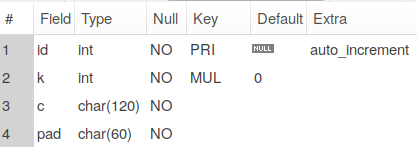
\includegraphics[scale = 0.6]{struktura_sbtest1.png}
	\label{fig:label}
\end{figure}

Aby wykonać test polecenie \textit{prepare} należy zamienić na polecenie \textit{run}. Przy takiej konfiguracji wykonywane jest następujące zapytanie:
\begin{spverbatim}
	SELECT c FROM sbtest1 WHERE id=?
\end{spverbatim}
\begin{figure}[H]
	\caption{Przykładowe statystyki testu wydajności izolowanych operacji odczytu.}
	\centering
	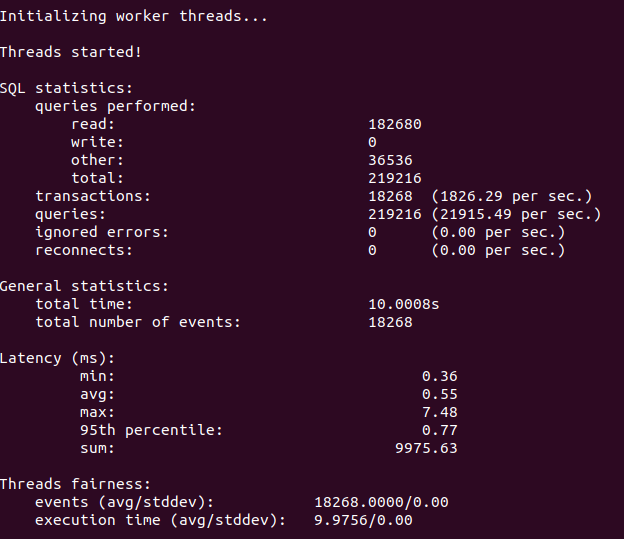
\includegraphics[scale = 0.6]{sysbench_statistics.png}
	\label{fig:label}
\end{figure}
\begin{center}
	\begin{tabular}{ | c | c | c | c | c | c |}
		\hline
		- & MyISAM & InnoDB & Memory & Archive & CSV  \\ 
		\hline
		średni czas [ms] & 0.54 & 0.55 & 0.38 & powyżej minuty & powyżej minuty \\
		\hline
	\end{tabular}
\end{center}
Silnik MEMORY okazał się najwydajniejszy w przypadku zapytania używającego pełnego klucza głównego. Dobry wynik wynika z faktu zastosowania indeksu HASH na kolumnie Id. Silniki InnoDB oraz MyISAM prezentują podobną wydajność w przypadku zapytań używających indeksy (w tym przypadku indeksy BTree). Silniki Archive oraz CSV wyraźnie odstają w tym zestawieniu ze względu na brak obsługi kluczy głównych.


\subsubsection{Symultaniczne operacje odczytu z wykorzystaniem klucza głównego oraz operacji zapisu.}

Do przygotowania testowych zestawów danych wykorzystałem następujące skrypty:
\begin{spverbatim}
	sysbench --db-driver=mysql --mysql-user=root --mysql-password=root --mysql-db=test --table_size=2000000 --num-threads=12 --range_selects=off --mysql_storage_engine=<nazwa silinika>  /usr/share/sysbench/oltp_read_write.lua prepare
\end{spverbatim}

Wykonanie testu analogicznie jak w poprzednich przypadkach wykonałem, zastępując słowo kluczowe \textit{prepare} na \textit{run}.

Przykładowe wynik polecenia został przedstawiony poniżej.
\begin{figure}[H]
	\caption{Przykładowe statystyki testu symultanicznych odczytów i zapisów.}
	\centering
	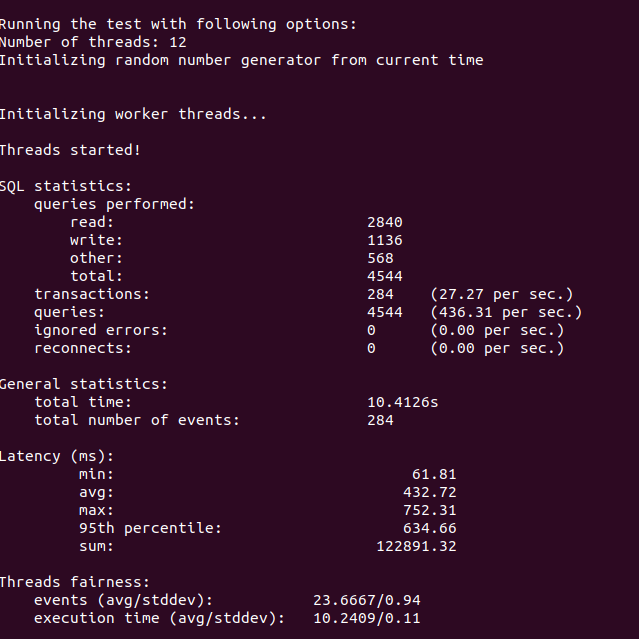
\includegraphics[scale = 0.6]{wyniki_testu_symulatnicznych_odczytow.png}
	\label{fig:label}
\end{figure}
\begin{center}
	\begin{tabular}{ | c | c | c | c | c | c |}
		\hline
		- & MyISAM & InnoDB & Memory & Archive & CSV  \\ 
		\hline
		średni czas [ms] & 432.7 & 75.5 & 425.1 & powyżej minuty & powyżej minuty \\
		\hline
	\end{tabular}
\end{center}
Widzimy, że w porównaniu z poprzednim testem, tym razem równolegle z operacjami odczytu wykonywane były operacje zapisu do tabeli. Wyniki testu zostały przedstawione w poniższej tabeli. W teście zdecydowanie najwydajniejszym silnikiem okazał się InnoDB, na co wpływ miał mechanizm blokowania pojedynczych rekordów, zamiast całej tabeli.

\subsubsection{Wyszukiwanie danych z zakresu.}

Do wykonania testu użyłem następującego polecenia:
\begin{spverbatim}
	sysbench --db-driver=mysql --mysql-user=root --mysql-password=root --mysql-db=test --table_size=2000000 --mysql_storage_engine=<nazwa silniku> --num-threads=12 /usr/share/sysbench/select_random_ranges.lua prepare
\end{spverbatim}
W związku z tym, że domyślnym indeksem dla tabeli MEMORY jest indeks HASH, a nie B-tree, na stworzonej tabeli stworzyłem dodatkowy indeks typu B-tree za pomocą polecenia:
\begin{spverbatim}
	CREATE INDEX k_12 on sbtest1(k) USING btree;
\end{spverbatim}
\begin{center}
	\begin{tabular}{ | c | c | c | c | c | c |}
		\hline
		- & MyISAM & InnoDB & Memory & Archive & CSV  \\ 
		\hline
		średni czas [ms] & 1.23 & 1.25 & 0.51 & 26687 & 51400 \\
		\hline
	\end{tabular}
\end{center}

Tym razem skuteczne okazały się tylko silniki wykorzystujące indeksy typu B-Tree, które pozwalają w optymalny sposób wyszukiwać za pomocą zakresu. Silnik \textit{MEMORY} okazał się najszybszy ze względu na przechowywanie danych bezpośrednio w pamięci.

\subsubsection{Operacje zapisu.}

Do wykonania testu użyłem następującego polecenia:
\begin{spverbatim}
	 sysbench --db-driver=mysql --mysql-user=root --mysql-password=root --mysql-db=test --table_size=2000000 --mysql_storage_engine=<nazwa silnika> --num-threads=12 /usr/share/sysbench/oltp_insert.lua prepare
\end{spverbatim}

Wyniki testu umieszcozne zostały w poniższej tabeli:
\begin{center}
	\begin{tabular}{ | c | c | c | c | c | c |}
		\hline
		- & MyISAM & InnoDB & Memory & Archive & CSV  \\ 
		\hline
		średni czas [ms] & 107.8 & 37.9 & 104.1 & 17.1 & 108.9 \\
		\hline
	\end{tabular}
\end{center}

W teście najszybszy okazał się silnik \textit{Archive}, który został zaprojektowany właśnie do wydajnego zapisywania danych. Duży wpływ na dużą wydajność ma bez wątpienia fakt braku indeksów. Istotnym jest również fakt niemal trzykrotnie większej wydajności operacji zapisu w tabelach \textit{InnoDB} w porównaniu do \textit{MyISAM}.

\subsubsection{Operacje aktualizacji danych z wykorzystaniem indeksu.}

Do wykonania testu użyłem następującego polecenia:
\begin{spverbatim}
	sysbench --db-driver=mysql --mysql-user=root --mysql-password=root --mysql-db=test --table_size=2000000 --num-threads=12 --mysql-storage_engine=
	<nazwa silnika> /usr/share/sysbench/oltp_update_index.lua prepare
\end{spverbatim}

Wyniki testu zamieściłem w poniższej tabeli:
\begin{center}
	\begin{tabular}{ | c | c | c | c | c | c |}
		\hline
		- & MyISAM & InnoDB & Memory & Archive & CSV  \\ 
		\hline
		średni czas [ms] & 109.1 & 54.9 & 105.9 & Brak wsparcia & Brak indeksów \\
		\hline
	\end{tabular}
\end{center}

Test był miarodajny jedynie dla trzech silników wspierających indeksy. Podstawową różnicą, która spowodowała niemal dwukrotnie większą wydajność operacji modyfikujących dane, jest mechanizm blokowania na poziomie rekordów, który pozwala tabelom \textit{InnoDB} działać wydajniej w środowisku wielowątkowym.

\subsubsection{Operacje aktualizacji danych bez wykorzystania indeksów.}
Do wykonania testu użyłem następującego polecenia:
\begin{spverbatim}
	sysbench --db-driver=mysql --mysql-user=root --mysql-password=root --mysql-db=test --table_size=2000000 --num-threads=12 --mysql-storage_engine=
	<nazwa silnika> /usr/share/sysbench/oltp_update_non_index.lua prepare
	
\end{spverbatim}
\begin{center}
	\begin{tabular}{ | c | c | c | c | c | c |}
		\hline
		- & MyISAM & InnoDB & Memory & Archive & CSV  \\ 
		\hline
		średni czas [ms] & 107.6 & 46.9 & 107.1 & Brak wsparcia & 67627.1 \\
		\hline
	\end{tabular}
\end{center}

Po raz kolejny w środowisku wielowątkowym silnik InnoDB okazał się najwydajniejszy przy wykonywaniu operacji modyfikująych dane. 
\subsubsection{Operacje usuwania danych}

\begin{spverbatim}
	sysbench --db-driver=mysql --mysql-user=root --mysql-password=root --mysql-db=test --table_size=2000000 --num-threads=12 --mysql-storage_engine=<nazwa tabeli>  /usr/share/sysbench/oltp_delete.lua prepare
\end{spverbatim}

\begin{center}
\begin{tabular}{ | c | c | c | c | c | c |}
	\hline
	- & MyISAM & InnoDB & Memory & Archive & CSV  \\ 
	\hline
	średni czas [ms] & 312.5 & 43.3 & 106.1 & Brak wsparcia & 62342.1 \\
	\hline
\end{tabular}

Silnik InnoDB jest najwydajniejszym rozwiązaniem ze względu na mechanizm blokowania na poziomie rekordów.
\end{center}


\subsubsection{Podsumowanie}

W tym rozdziale przedstawiłem podstawowe własności najpopularniejszych dostępnych obecnie silników MySQL. W zdecydowanej większości przypadków, które możemy spotkać we współczenych aplikacjach, korzystających z baz danych najlepszym rozwiązaniem jest silnik InnoDB. Są jednak specyficzne przypadki, kiedy dobrym wyborem może okazać się jeden z alternatywnych silników.